\section{Data Preprocessing}

\subsection{Text Cleaning}
Text cleaning is a crucial preprocessing step to ensure the quality and vectorization efficiency of the dataset. Our text cleaning procedures included:
\begin{itemize}
    \item Removal of URLs and email addresses to reduce noise.
    \item Replacement of newline characters with a space to maintain text continuity.
    \item Elimination of punctuation from a defined list, which included commonly used symbols such as:
    \begin{verbatim}
        !"#$%&'()*+,-./:;<=>?@[\]^_`{|}~“”¨«»®´·º½¾¿¡§£₤‘’
    \end{verbatim}
    \item Stripping of all unicode characters to standardize the text representation.
\end{itemize}

\subsection{Vectorization}
    \subsubsection{TF-IDF Embedding}
        The \texttt{TfidfVectorizer} from scikit-learn was employed to compute the Term Frequency-Inverse Document Frequency (TF-IDF) scores. These scores highlight the importance of words in relation to specific labels within the dataset. For instance in Figure \ref{fig:tfidf_scores}, the term "kill" registers a higher TF-IDF score under the "Threat" label, underscoring its relevance. This TF-IDF scoring mechanism informs the feature importance for our logistic regression and Naive Bayes SVM (NB-SVM) baseline models.

        \begin{figure}
            \centering
            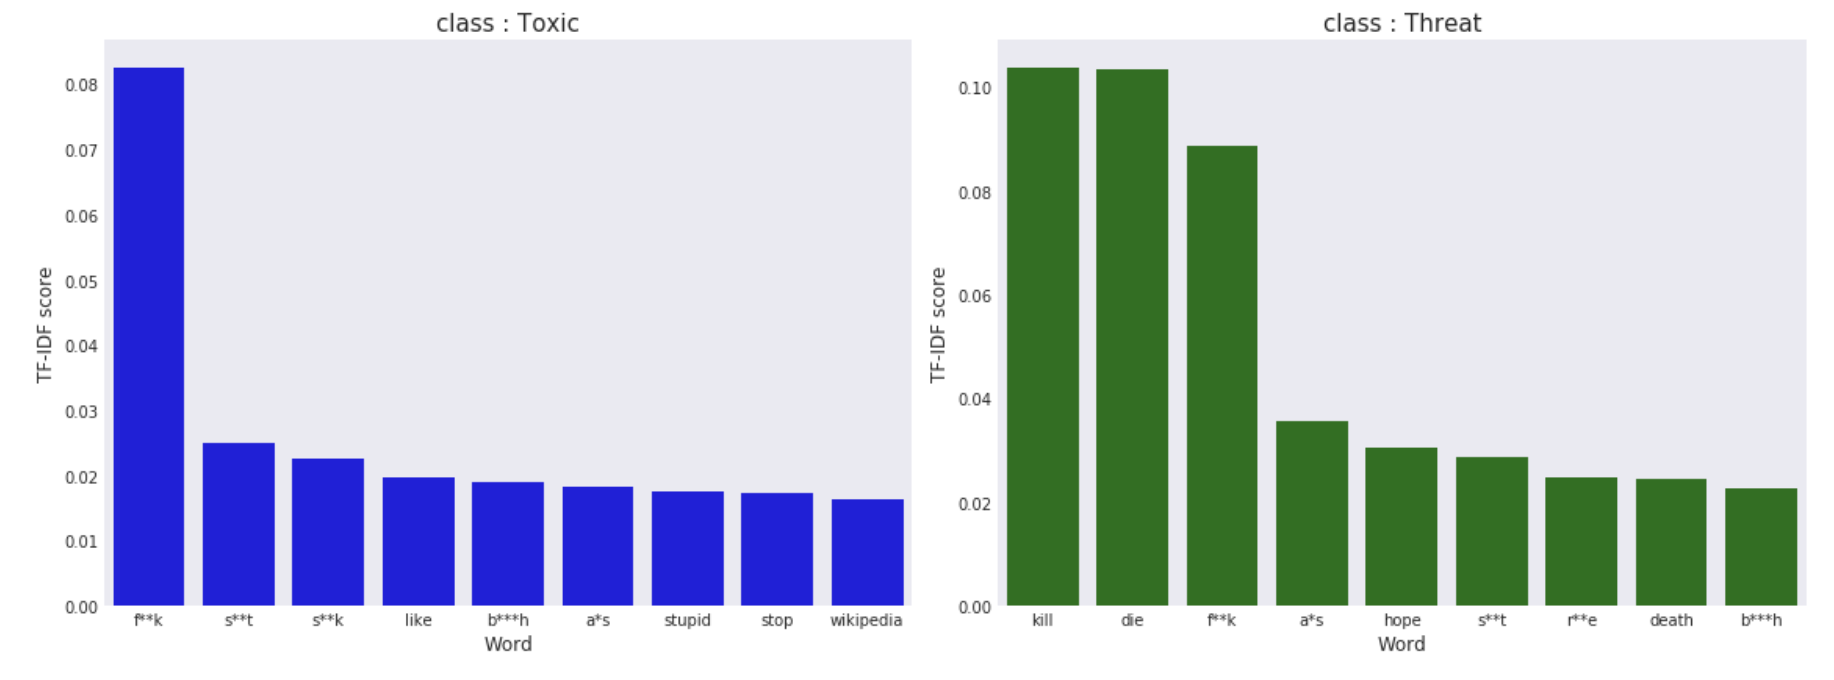
\includegraphics[width=0.6\textwidth]{images/data_analysis/TFIDF_WordCount.png}
            \caption{TF-IDF scores for select words within comments labeled Toxic or Threat.}
            \label{fig:tfidf_scores}
        \end{figure}

    \subsubsection{Tokenization}
        Tokenization prepares text for model inputs. We utilized the Keras tokenizer for LSTM and HuggingFace's tokenizer for BERT, with the following configurations:
        \begin{itemize}
            \item The Keras tokenizer's vocabulary was capped at the top 20,000 words to encompass the most relevant terms.
            \item We limited sequence lengths to 200 characters, capturing over 85\% of the comments, thereby maintaining sufficient context.
            \item Comments shorter than the maximum length were padded to ensure uniform input size.
        \end{itemize}

        \begin{figure}
            \centering
            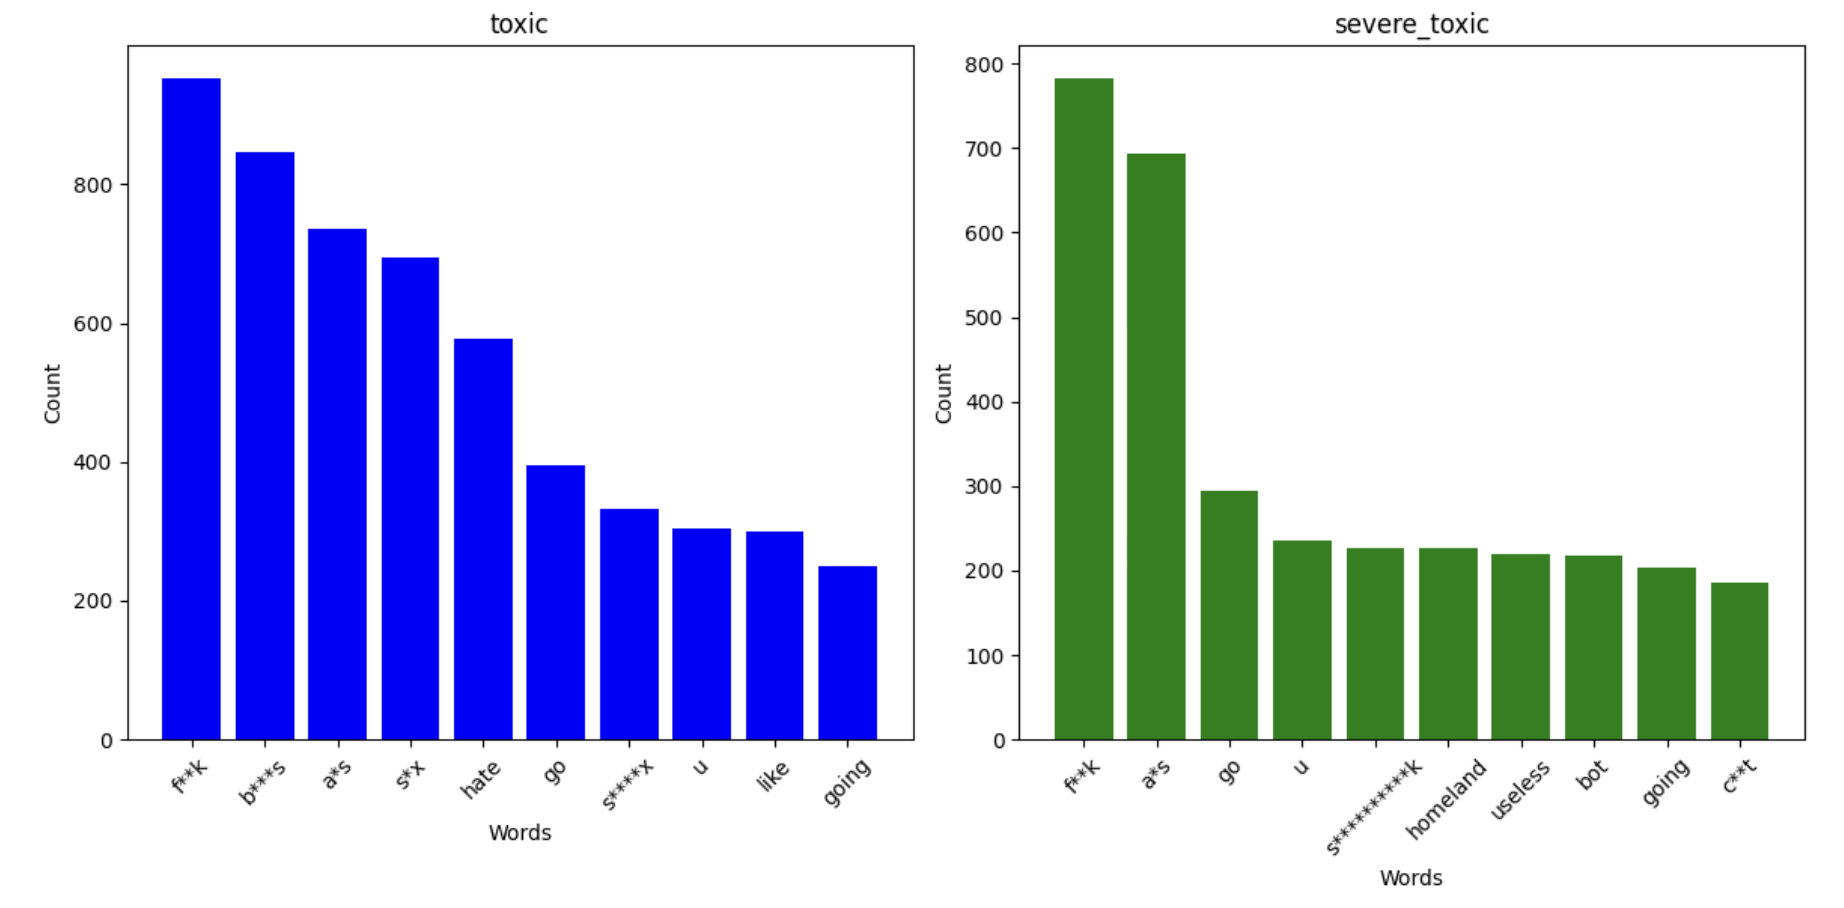
\includegraphics[width=0.6\textwidth]{images/data_analysis/LSTM_WordCount.png}
            \caption{Distribution of token counts from Keras Tokenizer for comments labeled Toxic or Threat.}
            \label{fig:token_counts}
        \end{figure}
